\documentclass{jthesis}

\usepackage{amsfonts}
\usepackage{amsmath}
\usepackage{geometry}
\usepackage{amsthm}
\usepackage{mathrsfs}
\usepackage{setspace}
\usepackage{footmisc}
\usepackage{hyperref}
\usepackage[dvipsnames]{xcolor}
\usepackage{graphicx}
\usepackage{subcaption}
\usepackage{amssymb}
\usepackage{listings}

\definecolor{codegreen}{rgb}{0,0.6,0}
\definecolor{codegray}{rgb}{0.5,0.5,0.5}
\definecolor{codepurple}{rgb}{0.58,0,0.82}
\definecolor{backcolour}{rgb}{0.95,0.95,0.92}
 
\lstdefinestyle{mystyle}{
    emph={self, Equation, loop, BlackHole2D,__init__, initialize, BlackHole, Application, Group},
    emphstyle=\color{PineGreen},
    commentstyle=\color{blue},
    keywordstyle={\color{BrickRed}\bfseries},
    numberstyle=\color{codegray},
    stringstyle=\color{codepurple},
    breakatwhitespace=false,         
    breaklines=true,                 
    captionpos=b,                    
    keepspaces=true,                 
    numbers=left,                    
    numbersep=5pt,                  
    showspaces=false,                
    showstringspaces=false,
    showtabs=false,                  
    tabsize=2
}

\title{The Effects of a Primordial Black Hole on the Surface of a Neutron Star} %Don't put a line break in, it gets really upset
\author{Brady Metherall}
\date{March 31, 2017}

\setlength\parindent{0pt}

\DeclareMathOperator{\sgn}{sgn}
\DeclareMathOperator{\Heavi}{H}

\DeclareMathOperator{\Hsign}{\mathscr{H}}
\newcommand\Hank[2][]{{\left( \Hsign_{#1} #2 \right) }}

\DeclareMathOperator{\grad}{\overset{\rightharpoonup}\nabla}

\newtheorem{theorem}{Theorem}[chapter]
\newtheorem{definition}[theorem]{Definition}
\newtheorem{corollary}[theorem]{Corollary}
\newtheorem{lemma}[theorem]{Lemma}

\renewcommand{\thefootnote}{\fnsymbol{footnote}}
\renewcommand\floatpagefraction{0.1}

\newcommand\numberthis{\addtocounter{equation}{1}\tag{\theequation}}

\begin{document}

\pagenumbering{roman}
\maketitle

\makeabstract{
The identity of dark matter has piqued the interest of astrophysicists for quite some time. One of the possible candidates is primordial black holes, black holes possibly created by perturbations in the very early universe. Observations can put estimates on the mass ranges and number of primordial black holes in the universe which can determine their contribution to dark matter, as well as the conditions in the very early universe. In this thesis the effects a primordial black hole has on the surface of a neutron star if they were to collide is investigated. Neutron stars are treated as a flat infinite incompressible fluid in this toy model. The shape of the surface waves created, and the energy deposited into the neutron star, are found both analytically and with simulations.
}

\makeacknowledgements{
First and most importantly, I would like to thank my supervisor and mentor Dr. Joseph MacMillan for his assistance, guidance, and inspiration over the past four years, and especially the last eight months. \\

Next, I would like to express my gratitude to Dr. Sean Bohun, Dr. Mihai Beligan, and Dr. Mehran Ebrahimi for offering their assistance to help me solve difficult differential equations and mathematical proofs. As well as Dr. Hendrick de Haan for allowing me use of Polar for conducting my simulations. I would also like to thank my fellow physics students for helping make the last four years enjoyable. \\

Lastly, I would like to thank my mom and dad, and grandparents for their endless support and encouragement over the past four years.
}

\makedeclaration

\maketableofcontents

\pagenumbering{arabic}

\doublespacing
\linespread{2}
\lstset{style=mystyle}

\documentclass[12pt]{report}

\usepackage{amsfonts}
\usepackage{amsmath}
\usepackage{geometry}
\usepackage{setspace}
%\usepackage{xcolor,graphicx}
%\usepackage{wrapfig}
%\usepackage{subcaption}
%\usepackage{hyperref}

\newgeometry{margin=1in}
\setlength\parindent{0pt}

\begin{document}

\doublespacing
\linespread{2}

\chapter{Introduction}

\section{Dark Matter and Primordial Black Holes}

\section{Literature Review}

\section{Model}

\section{Outline}

\end{document}


\documentclass[10pt]{article}

\usepackage{amsfonts}
\usepackage{amsmath}
\usepackage{geometry}
\usepackage{amsthm}
\usepackage{mathrsfs}
%\usepackage{xcolor,graphicx}
%\usepackage{wrapfig}
%\usepackage{subcaption}
%\usepackage{hyperref}

\newgeometry{margin=1in}
\setlength\parindent{0pt}

\DeclareMathOperator{\sgn}{sgn}
\DeclareMathOperator{\Heavi}{H}

\DeclareMathOperator{\Hsign}{\mathscr{H}}
\newcommand\Hank[2][0]{{(\Hsign_{#1} #2 ) }}

\newtheorem{theorem}{Theorem}[section]
\newtheorem{definition}[theorem]{Definition}
\newtheorem{corollary}[theorem]{Corollary}

\begin{document}

\section{Operators and Integral Transforms}
\begin{definition}[Operator]
\label{def:operator}
Let $A$, and $B$ be vector spaces with respective subspaces, $X$, and $Y$. An operator $\mathcal{T}$, maps any $x \in X$ to $Y$, and is denoted by $\mathcal{T}(x)$.
\end{definition}
Common examples of operators are the Sturm-Liouville operator, the Laplacian, or Hamiltonian. Our focus will be on the integral operator, or transform. Let the domain, and co-domain of the transform be $C[a,b]$ and $K: \mathbb{R}^2 \rightarrow \mathbb{R}$, then we can define our operator $\mathcal{T}:C[a,b] \rightarrow C[a,b]$ as
\begin{align*}
(\mathcal{T}f)(x) = \int_a^b f(y) K(x,y)dy,
\end{align*}
where $K$ is called the kernel function.

\begin{theorem}
\label{thm:continuity}
$\mathcal{T}f$ is continuous iff $\int_a^b |f(y)| dy < \infty$, and $K(x,y)$ is uniformly continuous on $[a,b]$.
\end{theorem}
\begin{proof}
For all $\epsilon > 0$, choose $\delta : |x - x_0| < \delta$, so that $|K(x,y) - K(x_0,y)| < \epsilon/M$, with $M = \int_a^b |f(y)| dy$. $\mathcal{T}f$ is continuous iff
\begin{align*}
|(\mathcal{T}f)(x) - (\mathcal{T}f)(x_0)| &= \left| \int_a^b K(x,y)f(y) dy - \int_a^b K(x_0,y)f(y) dy \right| \\
&\leq \int_a^b |K(x,y) - K(x_0,y)||f(y)| dy \\
&< \int_a^b \frac{\epsilon}{M} |f(y)| dy \\
&< \epsilon
\end{align*}
\end{proof}

\begin{corollary}
The conditions for Theorem \ref{thm:continuity} are satisfied if $a$ and $b$ are finite, as well as if $f$ and $K$ are bounded and continuous.
\end{corollary}
\begin{proof}
A bounded continuous function is integrable over a compact domain.
\end{proof}

\subsection{Hankel Transform}

\begin{definition}[Hankel Transform]
\label{def:hanktrans}
The Hankel transform of a function $f(s)$ is given by
\begin{align*}
\Hank[\nu]{f}(\sigma) = \int_0^\infty f(s) J_\nu(s \sigma) s \, ds,
\end{align*}
where $J_\nu$ is the Bessel function of the first kind, of order $\nu \geq -\frac{1}{2}$, and $\sigma$ is a non-negative real variable.
\end{definition}

\begin{corollary}[Inverse Hankel Transform]
\label{def:invhanktrans}
The Hankel transform is self-reciprocal, that is, the inverse Hankel transform is also given by Definition \ref{def:hanktrans}.
\end{corollary}
\begin{proof}
The Hankel transform is self-reciprocal
\begin{align*}
\iff f(s) &= \int_0^\infty \Hank[\nu]{f}(\sigma) J_\nu(s \sigma) \sigma \, d\sigma \\
\iff f(s) &= \int_0^\infty \int_0^\infty f(s') J_\nu(s \sigma) s' \, ds' J_\nu(s \sigma) \sigma \, d\sigma \\
&= \int_0^\infty f(s') s' \int_0^\infty J_\nu(s' \sigma) J_\nu(s \sigma) \sigma \, d\sigma \, ds' \\
&= f(s),
\end{align*}
by the orthogonality of the Bessel functions.
\end{proof}

\newpage

\begin{align*}
\varphi = \int_0^\infty J_0(kr) e^{kz} T(t) dk \\
\left( \frac{\partial \varphi}{\partial t} + (g \eta + \Phi) \right) \bigg|_{z=0} = 0 \\
\left( \frac{\partial^2 \varphi}{\partial t^2} + g \frac{\partial \varphi}{\partial z} + \frac{\partial \Phi}{\partial t} \right) \bigg|_{z=0} = 0\\
\text{where }\Phi = \frac{-Gm}{\sqrt{r^2+(z-vt)^2}} \\
\varphi = \frac{Gmv}{g} \int_0^\infty \frac{J_0(kr)e^{kz}}{1+kv^2/g} \left(-\sgn(t)e^{-kv|t|} + 2 \Heavi (t)\cos(\omega_k t) \right)dk \\
\text{with } \omega_k^2=gk
\end{align*}

We must write the gravitational potential as an infinite sum of Bessel functions,
\begin{align*}
\frac{\partial \Phi}{\partial t}\bigg|_{z=0} &= \int_0^\infty a(k; t)J_0(k r)k \, dk \\
a(k; t) &= \int_0^\infty \frac{\partial \Phi}{\partial t}\bigg|_{z=0} J_0(k r) r \, dr \text{ *HT*} \\
a(k;t) &= Gmv^2tk \int_0^\infty \frac{ J_0(k r) r}{(r^2+v^2t^2)^{3/2}} dr \\
&= Gmv^2t \frac{1}{|vt|} e^{-k|vt|} \text{ *HT*} \\
&= Gmv \sgn(t)e^{-kv|t|}
\end{align*}
\begin{gather*}
\int_0^\infty J_0(kr)  \ddot{T}(t) dk + g \int_0^\infty k J_0(kr) T(t) dk + Gmv \int_0^\infty \sgn(t) e^{-kv|t|} J_0(kr)k \, dk = 0 \\
\int_0^\infty \left[ \frac{\ddot{T}(t)}{k} + gT(t) + Gmv \sgn(t) e^{-kv|t|} \right] J_0(kr) k \, dk = 0 \\
\frac{\ddot{T}(t)}{k} + gT(t) + Gmv \sgn(t) e^{-kv|t|} = \int_0^\infty 0 \times J_0(kr) r \, dr = 0 \text{ *HT*} \\
T(t) = A \cos(\omega_k t) + B \sin(\omega_k t) \text{ homogenous solution } t \geq 0 \\
\text{Assume } T(t) = C e^{\xi |t|} \text{ for the particular solution} \\
\implies C \left(\xi^2 \sgn^2(t) e^{\xi |t|} + gk e^{\xi |t|} \right) + Gmvk \sgn(t) e^{-kv|t|} = 0 \\
\implies \xi = -kv, \quad C = \frac{-Gmvk \sgn(t)}{k^2v^2 + gk} = \frac{Gmv}{g} \frac{-\sgn(t)}{1+kv^2/g} \\
\implies T(t) = \frac{Gmv}{g} \frac{1}{1+kv^2/g} \left( -\sgn(t) e^{-kv|t|} + \Heavi(t) \left( \widetilde{A} \cos(\omega_k t) + \widetilde{B} \sin(\omega_k t \right) \right) \\
T(t) \text{ must be at least of class } C^1 \implies \widetilde{A} = 2, \quad \widetilde{B} = 0 \\
\implies \varphi = \frac{Gmv}{g} \int_0^\infty \frac{J_0(kr)e^{kz}}{1+kv^2/g} \left(-\sgn(t)e^{-kv|t|} + 2H(t)\cos(\omega_k t) \right)dk
\end{gather*}













\end{document}


\documentclass[12pt]{article}

\usepackage{amsfonts}
\usepackage{amsmath}
\usepackage{geometry}
\usepackage{amsthm}
\usepackage{mathrsfs}
\usepackage{xcolor,graphicx}
\usepackage{subcaption}
\usepackage{setspace}

\newgeometry{margin=1in}
\setlength\parindent{0pt}

\DeclareMathOperator{\sgn}{sgn}
\DeclareMathOperator{\Heavi}{H}

\DeclareMathOperator{\Hsign}{\mathscr{H}}
\newcommand\Hank[2][]{{\left( \Hsign_{#1} #2 \right) }}

\newtheorem{theorem}{Theorem}[section]
\newtheorem{definition}[theorem]{Definition}
\newtheorem{corollary}[theorem]{Corollary}

\begin{document}

\doublespacing
\linespread{2}

\section{Analytic Solution}

Typically, in fluid dynamics, the scalar function known as the velocity potential denoted by $\varphi$, is what is desired. Once the velocity potential is known, the system is solved because  $\overset{\rightharpoonup}\nabla \varphi = \bf{u}$, and in the case of a free surface, the deformation of the surface can readily be found from the velocity potential as well. The velocity potential will be found in the coming sub-chapters, and then the energy deposited into the neutron star will be calculated.

\subsection{Eigenfunctions of the Laplacian}

The first step in analytically solving for the velocity potential will be to find the eigenfunctions of Laplace's equation, $\nabla^2 \varphi = 0$, since the velocity potential is conservative. Since this is a partial differential equation we will assume the solution is the product of univariate functions, $\varphi = f(r) g(\theta) h(z) T(t)$. Expanding the Laplacian for cylindrical systems gives 
\begin{align*}
\frac{1}{r}\frac{\partial}{\partial r} \left( r \frac{\partial \varphi}{\partial r} \right) + \frac{1}{r^2} \left( \frac{\partial^2 \varphi}{\partial \theta^2} \right) + \frac{\partial^2 \varphi}{\partial z^2} = 0.
\end{align*}

The temporal component can be divided out since the Laplacian does not involve time, and will be found later on. Substituting in our assumed form, and dividing by $\varphi$, yields
\begin{align}
\label{eq:laplaciansub}
\frac{1}{fr}\frac{\partial}{\partial r}(rf') + \frac{1}{r^2}\frac{g''}{g} + \frac{h''}{h} = 0.
\end{align}

Where primes denote the derivative with respect to the function's only variable. Notice that the function $h(z)$ has been separated from both $f(r)$, and $g(\theta)$, and since each function is univariate, it must be the case that the last term is constant,
\begin{align*}
\frac{h''}{h} = k^2.
\end{align*}

We cleverly force this constant to be positive to satisfy the boundary conditions, namely, that $h(-\infty) = 0$. The most general solution to this is of course exponentials,
\begin{align*}
h(z) = Ae^{kz} + Be^{-kz}.
\end{align*}

Since the velocity potential has to vanish at negative infinity, this is simplified to
\begin{align}
\label{eq:h}
h(z) = e^{kz},
\end{align}

without loss of generality we can assume the constant is one, since it can be absorbed into $T(t)$. By substituting in $k^2$ and multiplying through by $r^2$, \eqref{eq:laplaciansub} becomes
\begin{align}
\label{eq:laplacenoh}
\frac{r}{f}\frac{\partial}{\partial r} \left( rf' \right) + k^2r^2 + \frac{g''}{g} = 0,
\end{align}

and once again, $g(\theta)$ has been separated from $f(r)$, and so the last term must be constant --
\begin{align*}
\frac{g''}{g} = -\mu^2.
\end{align*}

The constant is forced to be negative since $g(\theta)$ is expected to be periodic, and not exponential. Of course, the general solution to this differential equation is 
\begin{align*}
g(\theta) = A \sin(\mu \theta) + B \cos(\mu \theta).
\end{align*}

However, our system is cylindrically symmetric; there is no way to differentiate one value of $\theta$ to another, thus, it is expected that $\varphi$ has no $\theta$ dependence, and consequentially, $g(\theta)$ must be constant, the only way this is satisfied is if $\mu = 0$, so that
\begin{align}
\label{eq:g}
g(\theta) = 1.
\end{align}

By substituting $\mu = 0$ into \eqref{eq:laplacenoh}, and multiplying through by $f$ we obtain
\begin{align*}
r \frac{\partial}{\partial r}(rf') + (k^2r^2 - 0^2)f = 0,
\end{align*}

which indeed is Bessel's differential equation of order $0$. Therefore,
\begin{align*}
f(r) = A J_0(kr) + B Y_0(kr),
\end{align*}

but, once again, $B$ must equal zero since $Y_0(0)$ is not finite which is unphysical. The radial part thus simplifies to
\begin{align}
\label{eq:f}
f(r) = J_0(kr).
\end{align}

By combining \eqref{eq:h}, \eqref{eq:g}, and \eqref{eq:f} we find that the velocity potential is 
\begin{align*}
\varphi \propto e^{kz}T(t)J_0(kr),
\end{align*}

where $k$ is the eigenvalues. Clearly though, the only restriction on $k$ is that it must be a non-negative real number, all of which are a valid solution to Laplace's equation. Therefore, the total solution must be the sum of all of these, or since $k$ is valid within an interval, we have the integral form 
\begin{align}
\label{eq:phieigen}
\varphi = \int_0^\infty e^{kz}T(t)J_0(kr)dk.
\end{align}

The temporal component can be solved for using equations of fluid dynamics.

\subsection{Temporal Component of the Velocity Potential}

***Add the part about the fluid dynamics equation*** \\

We must write the gravitational potential as an infinite sum of Bessel functions to match the form of $\varphi$, to do so, we take the Hankel transform,
\begin{align*}
\frac{\partial \Phi}{\partial t}\bigg|_{z=0} &=  \int_0^\infty \Hank{\frac{\partial \Phi}{\partial t}\bigg|_{z=0}}(k) J_0(kr) k \, dk \\
&= G m v^2 t \int_0^\infty \Hank{\frac{1}{(r^2 + v^2 t^2)^{3/2}}}(k) J_0(kr) k \, dk \footnote{hey} \\
&= G m v^2 t \int_0^\infty \frac{1}{|vt|} e^{-k|vt|} J_0(kr) k \, dk \\
&= G m v \sgn(t) \int_0^\infty e^{-kv|t|} J_0(kr) k \, dk.
\end{align*}
\footnotetext{Note that $\int_0^\infty \sqrt{r}(r^2 + v^2 t^2)^{-3/2} dr = \Gamma^2(3/4) (\pi v^3 t^3)^{-1/2} < \infty$ for $t \neq 0$ which is not concerning since this is true almost everywhere, and so the condition in Theorem *** is satisfied.}
We can now substitute this into *** to obtain,
\begin{align*}
\int_0^\infty J_0(kr)  \ddot{T}(t) dk + g \int_0^\infty k J_0(kr) T(t) dk + Gmv \int_0^\infty \sgn(t) e^{-kv|t|} J_0(kr)k \, dk = 0 \\
\text{or, } \int_0^\infty \left[ \frac{\ddot{T}(t)}{k} + gT(t) + Gmv \sgn(t) e^{-kv|t|} \right] J_0(kr) k \, dk = 0,
\end{align*}
but, this is nothing more than the Hankel transform of the differential equation for $T$. By taking the Hankel transform of both sides we can remove the integral,
\begin{align*}
\frac{\ddot{T}(t)}{k} + gT(t) + Gmv \sgn(t) e^{-kv|t|} = 0.
\end{align*}
Clearly, the homogeneous solution is $T(t) = A \cos(\omega_k t) + B \sin(\omega_k t)$ with $\omega_k^2 = gk$. The form of the differential equations suggests the form $T(t) = C e^{-kv|t|}$ for the particular solution. Substituting this in yields
\begin{align*}
C \left(k^2 v^2 \sgn^2(t) e^{-kv |t|} + gk e^{-kv |t|} \right) &+ Gmvk \sgn(t) e^{-kv|t|} = 0,
\end{align*}
giving
\begin{align*}
C &= \frac{-Gmvk \sgn(t)}{k^2v^2 + gk} \\
&= \frac{Gmv}{g} \frac{-\sgn(t)}{1+kv^2/g}
\end{align*}
as the coefficient, and,
\begin{align*}
T(t) = \frac{Gmv}{g} \frac{1}{1+kv^2/g} \left( -\sgn(t) e^{-kv|t|} \right) + A \cos(\omega_k t) + B \sin(\omega_k t)
\end{align*}
as the full time component of the velocity potential. We can now apply the boundary conditions to find $A$, and $B$. Physically, we expect $T(t) \in C^1(-\infty,\infty)$, furthermore, we only expect the sinusoidal terms to contribute at times greater than zero, thus,
\begin{align*}
T(t) &= \frac{Gmv}{g}\frac{1}{1+kv^2/g} \left(-\sgn(t)e^{-kv|t|} + 2H(t)\cos(\omega_k t) \right)dk, \text{ and,} \\
\varphi &= \frac{Gmv}{g} \int_0^\infty \frac{J_0(kr)e^{kz}}{1+kv^2/g} \left(-\sgn(t)e^{-kv|t|} + 2H(t)\cos(\omega_k t) \right)dk.
\end{align*}

\begin{align*}
\varphi = \int_0^\infty J_0(kr) e^{kz} T(t) dk \\
\left( \frac{\partial \varphi}{\partial t} + (g \eta + \Phi) \right) \bigg|_{z=0} = 0 \\
\left( \frac{\partial^2 \varphi}{\partial t^2} + g \frac{\partial \varphi}{\partial z} + \frac{\partial \Phi}{\partial t} \right) \bigg|_{z=0} = 0\\
\text{where }\Phi = \frac{-Gm}{\sqrt{r^2+(z-vt)^2}} \\
\varphi = \frac{Gmv}{g} \int_0^\infty \frac{J_0(kr)e^{kz}}{1+kv^2/g} \left(-\sgn(t)e^{-kv|t|} + 2 \Heavi (t)\cos(\omega_k t) \right)dk \\
\text{with } \omega_k^2=gk
\end{align*}

\newpage

\begin{figure}[p]
\begin{centering}
 \begin{subfigure}{\textwidth}
  \input{./Analytic000}
  \caption{$t=-1$ s.}
 \end{subfigure} \\
 \begin{subfigure}{\textwidth}
  \input{./Analytic001}
  \caption{$t=0$ s.}
 \end{subfigure} \\
 \begin{subfigure}{\textwidth}
  \input{./Analytic002}
  \caption{$t=1$ s.}
 \end{subfigure}
\end{centering}
\end{figure}

\begin{figure}[p] \ContinuedFloat
\begin{centering}
 \begin{subfigure}{\textwidth}
  \input{./Analytic003}
  \caption{$t=2$ s.}
 \end{subfigure} \\
 \begin{subfigure}{\textwidth}
  \input{./Analytic004}
  \caption{$t=3$ s.}
 \end{subfigure} \\
  \begin{subfigure}{\textwidth}
  \input{./Analytic005}
  \caption{$t=4$ s.}
 \end{subfigure}
 \end{centering}
\end{figure}




\end{document}


%\documentclass[12pt]{report}
%
%\usepackage{amsfonts}
%\usepackage{amsmath}
%\usepackage{geometry}
%\usepackage{listings}
%\usepackage[dvipsnames]{xcolor}
%\usepackage{graphicx}
%%\usepackage{wrapfig}
%\usepackage{subcaption}
%%\usepackage{hyperref}
%\usepackage{setspace}
%
%\definecolor{codegreen}{rgb}{0,0.6,0}
%\definecolor{codegray}{rgb}{0.5,0.5,0.5}
%\definecolor{codepurple}{rgb}{0.58,0,0.82}
%\definecolor{backcolour}{rgb}{0.95,0.95,0.92}
% 
%\lstdefinestyle{mystyle}{
%    emph={self, Equation, loop, BlackHole2D,__init__, initialize, BlackHole, Application, Group},
%    emphstyle=\color{PineGreen},
%    commentstyle=\color{blue},
%    keywordstyle={\color{BrickRed}\bfseries},
%    numberstyle=\color{codegray},
%    stringstyle=\color{codepurple},
%    breakatwhitespace=false,         
%    breaklines=true,                 
%    captionpos=b,                    
%    keepspaces=true,                 
%    numbers=left,                    
%    numbersep=5pt,                  
%    showspaces=false,                
%    showstringspaces=false,
%    showtabs=false,                  
%    tabsize=2
%}
%
%\newgeometry{margin=1in}
%\setlength\parindent{0pt}
%
%\DeclareMathOperator{\grad}{\overset{\rightharpoonup}\nabla}
%
%\begin{document}
%
%\doublespacing
%\linespread{2}
%\lstset{style=mystyle}

\chapter{Simulation Solution}
\label{chap:sim}

\section{Smoothed Particle Hydrodynamics}

Since we model neutron stars as a fluid in order to simulate the collision of a primordial black hole with a neutron star, we need to use computational fluid dynamics, more specifically, we shall use smoothed particle hydrodynamics (SPH). One of the biggest advantages of smoothed particle hydrodynamics is that it is mesh-free, unlike most computational fluid dynamics methods. Therefore, it is very useful for interactions between different types of particles and for free surface simulations. Smoothed particle hydrodynamics was initially developed in 1977 for simulating spherically asymmetric stars \cite{origsph}. A major assumption in the modelling of stars is that they are spherically symmetric, however, there are a lot of cases where this is not true. For example the collapse of a protostar will be very inhomogeneous, or if the star has a large angular momentum or strong magnetic fields, the star will be considerably deformed \cite{origsph}. \\

Smoothed particle hydrodynamics has since been extended more generally so it can be applied outside of astrophysics to areas such as solid mechanics and fluid dynamics. In essence, smoothed particle hydrodynamics uses similar methods of N-body code -- the continuous media is represented as a set of particles, and the equations are solved numerically. Mathematically, the particles represent the points at which the properties of the fluid are calculated, and the rest can then be interpolated. Physically, the particles are simply a subset of all the particles in the system \cite{newsph}. \\

Typically, smoothed particle hydrodynamics uses a nearest neighbour scheme for calculating the changes in a particle's properties. This is done by using a cubic Hermite spline to interpolate properties within a radius of twice the smoothing length of a particular particle. A cubic Hermite spline is a set of cubic polynomials specified by its values, and the values of its first derivative at the boundaries of the interval.

\subsection{PySPH}

The simulations were conducted with PySPH \cite{pysph}, open source SPH code written in Python and compiled in Cython. This allows a majority of the code to be written in pure Python, but is then converted to high performance Cython code to run at speeds closer to C and FORTRAN. For further optimizations, PySPH can run in parallel with OpenMP and MPI to take advantage of multiple cores / threads. One of the main reasons for choosing PySPH is that it allows the flexibility of user defined classes and equations which was needed to incorporate the primordial black hole.

\section{Code}

In order to simulate a primordial black hole collision with a neutron star we must first write a class to include the acceleration. The acceleration of course is just
\begin{align*}
\overset{\rightharpoonup}a &= - \frac{1}{m_{part}} \grad \Phi.
\end{align*}

Within the coordinates in PySPH
\begin{align*}
\overset{\rightharpoonup}a &= \frac{-m}{\left( x^2 + s^2 + (y + v\tau)^2 \right)^{3/2}} \left( \begin{matrix}
x \\
y+v \tau
\end{matrix}
\right)
\end{align*}
with $G = 1$, $\tau = t-t\_hit$, and $s$ a softening length so the solution does not diverge at $\tau = 0$ at the origin. The mass of the particle is also omitted in the simulation because PySPH uses acceleration per unit mass. In the class function (Figure \ref{fig:blackholeclass}) the velocity is hard coded to be $1$, and the parameter \emph{t\_hit} is used to offset the collision of the primordial black hole since the simulation starts at $t = 0$. \\

Now that the class function has been written, it can be called within the equations block of the main file, \emph{blackhole.py}. Figure \ref{fig:blackhole} shows the important sections of \emph{blackhole.py}; first the acceleration equation is imported, and the values for the simulation are specified in the preamble. Then, the black hole can be added to the equations group in the main acceleration block. The included example \emph{hydrostatic\_tank.py} was used as the base for \emph{blackhole.py}, it was the most useful starting point -- it is a 2D tank filled with fluid, and includes the force of gravity. \\

\begin{figure}[p]
\lstinputlisting[language=Python, lastline=18]{../BlackHoleEquation.py}
\caption[Acceleration addition due to a primordial black hole]{Class file for adding the acceleration due to the primordial black hole, \emph{BlackHoleEquation.py}.}
\label{fig:blackholeclass}
\end{figure}

\begin{figure}[p]
  \lstinputlisting[language=Python, firstnumber=19, firstline=19, lastline=21]{../blackhole.py}
  \lstinputlisting[language=Python, firstnumber=40, firstline=40, lastline=59]{../blackhole.py}
  \lstinputlisting[language=Python, firstnumber=82, firstline=82, lastline=82]{../blackhole.py}
  \lstinputlisting[language=Python, firstnumber=171, firstline=171, lastline=173]{../blackhole.py}
  \lstinputlisting[language=Python, firstnumber=194, firstline=194, lastline=195]{../blackhole.py}
  \lstinputlisting[language=Python, firstnumber=212, firstline=212, lastline=217]{../blackhole.py}
 \caption[Modifications of the hydrostatic tank example, \emph{blackhole.py}]{Modifications of the hydrostatic tank example, \emph{blackhole.py}.}
 \label{fig:blackhole}
\end{figure}

The parameters of the simulation were mostly the same as what were used to generate the images of the analytic solution -- everything set equal to unity -- with the exceptions of \emph{t\_hit} $= 200$, and $s=0.01$. The reason \emph{t\_hit} is so large is due to how the particles are initially placed. They are simply placed on a grid with spacing $dx$; once the simulation starts, gravity pulls the surface down attempting to equilibrate to a linear pressure gradient. However, since the fluid is not at equilibrium, the surface undergoes harmonic motion and is slowly dampened to equilibrium and so the long \emph{t\_hit} is an attempt to dampen out a majority of the oscillations. \\

Determining the dimensions of the tank required a considerable amount of care. If the tank was too narrow, the walls at the edges would reflect the initial waves which would then start to interfere with the secondary waves. This caused erroneous results in the energy calculations during testing. Similarly, if the tank was too shallow, the waves resembled shallow water waves instead of deep, as in our model. And of course, if the tank was needlessly large, it greatly affected the computation time of the simulation. In the end, $Lx = 120$, $Ly = 15$, and $dx = 0.075$ were decided on.

\section{Simulation Results}

In total the simulation took about 330 CPU hours over the course of three days. The resulting surface waves from the collision can be seen in Figure \ref{fig:simresults}.
\begin{figure}[p]
\centering
\begin{subfigure}{\textwidth}
\input{./4Simulation/Sim199}
\caption{$\tau = -1$}
\end{subfigure} \\
\begin{subfigure}{\textwidth}
\input{./4Simulation/Sim200}
\caption{$\tau = 0$}
\end{subfigure} \\
\begin{subfigure}{\textwidth}
% GNUPLOT: LaTeX picture with Postscript
\begingroup
  \makeatletter
  \providecommand\color[2][]{%
    \GenericError{(gnuplot) \space\space\space\@spaces}{%
      Package color not loaded in conjunction with
      terminal option `colourtext'%
    }{See the gnuplot documentation for explanation.%
    }{Either use 'blacktext' in gnuplot or load the package
      color.sty in LaTeX.}%
    \renewcommand\color[2][]{}%
  }%
  \providecommand\includegraphics[2][]{%
    \GenericError{(gnuplot) \space\space\space\@spaces}{%
      Package graphicx or graphics not loaded%
    }{See the gnuplot documentation for explanation.%
    }{The gnuplot epslatex terminal needs graphicx.sty or graphics.sty.}%
    \renewcommand\includegraphics[2][]{}%
  }%
  \providecommand\rotatebox[2]{#2}%
  \@ifundefined{ifGPcolor}{%
    \newif\ifGPcolor
    \GPcolorfalse
  }{}%
  \@ifundefined{ifGPblacktext}{%
    \newif\ifGPblacktext
    \GPblacktexttrue
  }{}%
  % define a \g@addto@macro without @ in the name:
  \let\gplgaddtomacro\g@addto@macro
  % define empty templates for all commands taking text:
  \gdef\gplbacktext{}%
  \gdef\gplfronttext{}%
  \makeatother
  \ifGPblacktext
    % no textcolor at all
    \def\colorrgb#1{}%
    \def\colorgray#1{}%
  \else
    % gray or color?
    \ifGPcolor
      \def\colorrgb#1{\color[rgb]{#1}}%
      \def\colorgray#1{\color[gray]{#1}}%
      \expandafter\def\csname LTw\endcsname{\color{white}}%
      \expandafter\def\csname LTb\endcsname{\color{black}}%
      \expandafter\def\csname LTa\endcsname{\color{black}}%
      \expandafter\def\csname LT0\endcsname{\color[rgb]{1,0,0}}%
      \expandafter\def\csname LT1\endcsname{\color[rgb]{0,1,0}}%
      \expandafter\def\csname LT2\endcsname{\color[rgb]{0,0,1}}%
      \expandafter\def\csname LT3\endcsname{\color[rgb]{1,0,1}}%
      \expandafter\def\csname LT4\endcsname{\color[rgb]{0,1,1}}%
      \expandafter\def\csname LT5\endcsname{\color[rgb]{1,1,0}}%
      \expandafter\def\csname LT6\endcsname{\color[rgb]{0,0,0}}%
      \expandafter\def\csname LT7\endcsname{\color[rgb]{1,0.3,0}}%
      \expandafter\def\csname LT8\endcsname{\color[rgb]{0.5,0.5,0.5}}%
    \else
      % gray
      \def\colorrgb#1{\color{black}}%
      \def\colorgray#1{\color[gray]{#1}}%
      \expandafter\def\csname LTw\endcsname{\color{white}}%
      \expandafter\def\csname LTb\endcsname{\color{black}}%
      \expandafter\def\csname LTa\endcsname{\color{black}}%
      \expandafter\def\csname LT0\endcsname{\color{black}}%
      \expandafter\def\csname LT1\endcsname{\color{black}}%
      \expandafter\def\csname LT2\endcsname{\color{black}}%
      \expandafter\def\csname LT3\endcsname{\color{black}}%
      \expandafter\def\csname LT4\endcsname{\color{black}}%
      \expandafter\def\csname LT5\endcsname{\color{black}}%
      \expandafter\def\csname LT6\endcsname{\color{black}}%
      \expandafter\def\csname LT7\endcsname{\color{black}}%
      \expandafter\def\csname LT8\endcsname{\color{black}}%
    \fi
  \fi
    \setlength{\unitlength}{0.0500bp}%
    \ifx\gptboxheight\undefined%
      \newlength{\gptboxheight}%
      \newlength{\gptboxwidth}%
      \newsavebox{\gptboxtext}%
    \fi%
    \setlength{\fboxrule}{0.5pt}%
    \setlength{\fboxsep}{1pt}%
\begin{picture}(8640.00,3600.00)%
    \gplgaddtomacro\gplbacktext{%
      \csname LTb\endcsname%
      \put(682,967){\makebox(0,0)[r]{\strut{}$-4$}}%
      \put(682,1493){\makebox(0,0)[r]{\strut{}$-2$}}%
      \put(682,2020){\makebox(0,0)[r]{\strut{}$0$}}%
      \put(682,2546){\makebox(0,0)[r]{\strut{}$2$}}%
      \put(682,3072){\makebox(0,0)[r]{\strut{}$4$}}%
      \put(814,484){\makebox(0,0){\strut{}$-10$}}%
      \put(2383,484){\makebox(0,0){\strut{}$-5$}}%
      \put(3952,484){\makebox(0,0){\strut{}$0$}}%
      \put(5521,484){\makebox(0,0){\strut{}$5$}}%
      \put(7090,484){\makebox(0,0){\strut{}$10$}}%
    }%
    \gplgaddtomacro\gplfronttext{%
      \csname LTb\endcsname%
      \put(176,2019){\makebox(0,0){\strut{}$y$}}%
      \put(3952,154){\makebox(0,0){\strut{}$x$}}%
      \csname LTb\endcsname%
      \put(7692,704){\makebox(0,0)[l]{\strut{}$0.99$}}%
      \put(7692,1142){\makebox(0,0)[l]{\strut{}$1$}}%
      \put(7692,1581){\makebox(0,0)[l]{\strut{}$1.01$}}%
      \put(7692,2019){\makebox(0,0)[l]{\strut{}$1.02$}}%
      \put(7692,2458){\makebox(0,0)[l]{\strut{}$1.03$}}%
      \put(7692,2896){\makebox(0,0)[l]{\strut{}$1.04$}}%
      \put(7692,3335){\makebox(0,0)[l]{\strut{}$1.05$}}%
      \put(8286,2019){\makebox(0,0){\strut{} $\rho$}}%
    }%
    \gplbacktext
    \put(0,0){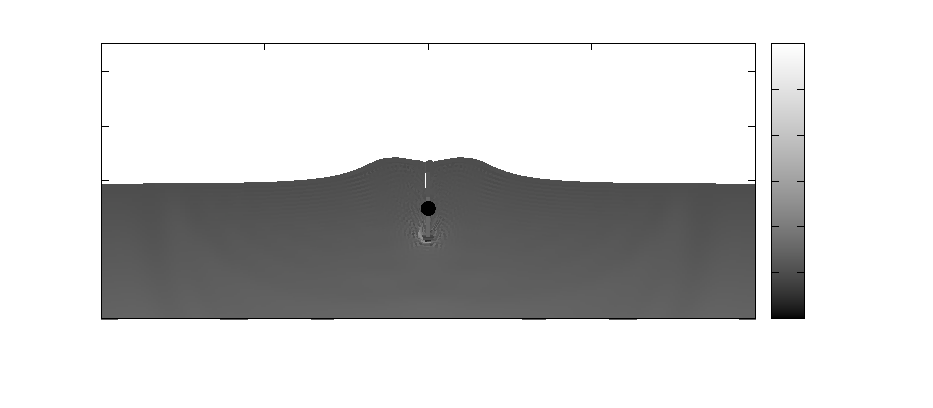
\includegraphics{./4Simulation/Sim201}}%
    \gplfronttext
  \end{picture}%
\endgroup

\caption{$\tau = 1$}
\end{subfigure}
\end{figure}
\begin{figure}[p] \ContinuedFloat
\centering
\begin{subfigure}{\textwidth}
\input{./4Simulation/Sim202}
\caption{$\tau = 2$}
\end{subfigure} \\
\begin{subfigure}{\textwidth}
\input{./4Simulation/Sim205}
\caption{$\tau = 5$}
\end{subfigure} \\
\begin{subfigure}{\textwidth}
\input{./4Simulation/Sim210}
\caption{$\tau = 10$}
\end{subfigure}
\caption[Surface waves resulting from the simulation]{Surface waves resulting from the simulation.  The full animation can be found at \url{https://github.com/bmetherall/Primordial_Black_Holes/blob/master/Videos/Simulation.gif}.}
\label{fig:simresults}
\end{figure}
As with the analytic results, we see that the surface of the neutron star pulls upwards before the collision due to the gravitational force of the primordial black hole. Then, after the collision, the initial wave propagates outwards. It is fairly difficult to notice, however, a second much smaller amplitude wave is created as well. Unfortunately, because of the resolution of the simulation, waves smaller than $dx$ cannot be seen, unlike in the analytic solution which had a much smaller spacing. \\

In order to calculate the energy we do so in the traditional way, by taking the sum of the potential and kinetic energies of each particle,
\begin{align*}
E &= \sum_i T_i + U_i, \\
&= \sum_i \frac{1}{2} m_i \left( u_i^2 + v_i^2 \right) + m_i g y_i.
\end{align*}
However, to compare to the analytic result, we must transform this into three dimensions by revolving about the $y$ axis. This can be done by weighting each particle by $\pi |x_i| / dx$,
\begin{align*}
E &= \frac{\pi}{dx} \sum_i \left( \frac{1}{2} \left( u_i^2 + v_i^2 \right) + g y_i \right) m_i |x_i|.
\end{align*}

\begin{figure}
\centering
\begin{subfigure}{\textwidth}
\input{./4Simulation/BadEnergy}
\caption{Raw energy data; this is very noisy because of the oscillations of the surface.}
\label{fig:badenergy}
\end{subfigure} \\
\begin{subfigure}{\textwidth}
\input{./4Simulation/GoodEnergy}
\caption{Smoothed energy without noise.}
\label{fig:goodenergy}
\end{subfigure}
\caption[Energy transfer from the simulation]{Energy transfer from the simulation.}
\end{figure}

This is essentially the same as a shell integration, however, we only integrate through $\pi$, and the absolute value of the $x$ coordinate is needed. The energy is calculated in this fashion for all time steps and is plotted in Figure \ref{fig:badenergy}. Clearly, this is of little use since the energy is full of noise and highly oscillatory. As mentioned before, this is also the result of how the particles are initially placed within the simulation. As the surface oscillates up and down while attempting to equilibrate, so too does the potential energy. The oscillations have a period of 39 time steps, and therefore, by taking running averages of 39 time steps, most of the noise is removed. Also for clarity, the damping is removed, and the energy has been shifted to start at 0; the resulting plot is much cleaner and is in Figure \ref{fig:goodenergy}. \\

This cleaned up energy has a very similar shape to the analytic calculation; initially, the neutron star gains energy as the primordial black hole approaches. And after the collision there is a large peak in the energy similar to the analytic solution. However, this jump in energy is much larger. Furthermore, at approximately $\tau = 40$ the initial wave hits the boundaries which causes the energy of the system to increase as the wave climbs the wall. After this, the wave is reflected back towards the centre of the tank. This also causes the first wave to interfere with the smaller waves trailing it which again causes the energy to increase -- this is the main cause of the erratic behaviour of the energy at times greater than 40. \\

Another point of interest is that since the tank has a depth of $15$, at $\tau = 15$ the primordial black hole exits the tank. During the lower resolution testing this did not appear to affect the results of the simulation, however, it indeed does. As the primordial black hole exits the tank a shock wave is created. In Figure \ref{fig:shock} the shock wave can be seen moving outwards from the bottom of the tank, and when it reaches the surface, it is reflected back into the star. Given the speed of the shock wave and the dimensions of the tank, it will be dampened out within a few time units and does not appear to effect the energy of the system.

\begin{figure}
\centering
\begin{subfigure}{\textwidth}
\input{./4Simulation/Shock1}
\caption{Initial shock-wave. $\tau  = 15.24$.}
\end{subfigure} \\
\begin{subfigure}{\textwidth}
\input{./4Simulation/Shock2}
\caption{Reflected shock-wave. $\tau = 15.56$.}
\end{subfigure}
\caption[Shock-wave created by primordial black hole leaving tank]{Shock-wave created by primordial black hole leaving tank.}
\label{fig:shock}
\end{figure}

%\end{document}


\chapter{Conclusions}
\label{chap:conc}

In this thesis we looked at the effect a primordial black hole has on the surface of a neutron star if the primordial black hole were to pass through the neutron star. To simplify the problem we first assume that a neutron star is an infinite plane, and that primordial black holes are point masses. One of the main results was analytically showing that the energy transfer in this model is
\begin{align*}
E &= 4 \pi \rho \frac{G^2 m^2}{g}.
\end{align*}
We also independently simulated the collision with smoothed particle hydrodynamics. The profile of the energy transfer matched similarly in both cases, however, in the simulation there was several disturbances in the energy skewing the shape. \\

If we were to further develop this work, there are a few obvious modifications, and extensions. Firstly, there are better methods of simulating the collision so that the fluid is started at equilibrium to stop the oscillations of the surface, and so the walls of the tank do not reflect the waves back into the centre. The next step to improve the result would be moving from an infinite plane to a spherical star, to better match reality. Defillon, Granet, Tinyakov, and Tytgat \cite{tidalcapture} investigated the spherical case as well, as the flat star, however, within the time constraints of this thesis, it was not looked at in great detail. \\

Finally, to obtain the most precise estimates of the energy transfer between a primordial black hole and a neutron star -- and what may be observed here on Earth -- much more sophisticated physics needs to be incorporated. For example, a group in Illinois uses full general relativistic magnetohydrodynamics (GRMHD) code to simulate events such as black hole mergers, or gravitational waves \cite{nuts}.

\begin{thebibliography}{99}

\bibitem{fluids}
D. J. Acheson, \emph{Elementary Fluid Dynamics}, Oxford University Press, 1990.

\bibitem{massrange}
A. Barrau, D. Blais, G. Boudoul, D. Polarski, \emph{Peculiar Relics from Primordial Black Holes in the Inflationary Paradigm}, Annalen der Physik 13, 2003.

\bibitem{dynamicalfriction}
Fabio Capela, Maxim Pshirkov, and Peter Tinyakov, \emph{Constraints on Primordial Black Holes as Dark Matter Candidates from Capture by Neutron Stars}, American Physics Society Phys. Rev. D 87, 2013.

\bibitem{massheavy}
B. J. Carr, and M. Sakellariadou, \emph{Dynamical Constraints on Dark Matter in Compact Objects}, The Astrophysical Journal 516, 1999.

\bibitem{bigpaper}
Bernard Carr, Florian K{\"u}hnel, and Marit Sandstad, \emph{Primordial Black Holes as Dark Matter}, American Physical Society Phys. Rev. D 94, 2016.

\bibitem{cousin}
Pierre Cousin, \emph{Sur les Fonctions de $n$ Variables Complexes}, Acta Math. 19, 1895.

\bibitem{critdens}
Richard H. Cyburt, Brian D. Fields, Keith A. Olive, \emph{Primordial Nucleosynthesis in Light of WMAP}, Harvard Colloquia, 2003.

\bibitem{transforms}
Lokenath Debnath, and Dambaru Bhatta, \emph{Integral Transforms and Their Applications}, Chapman \& Hall/CRC, 2007.

\bibitem{tidalcapture}
Guillaume Defillon, Etienne Granet, Peter Tinyakov, and Michel H.G. Tytgat, \emph{On Tidal Capture of Primordial Black Holes by Neutron Stars}, American Physics Society Phys. Rev. D 90, 2014.

\bibitem{merger}
Zachariah B. Etienne, Joshua A. Faber, Yuk Tung Liu, Stuart L. Shapiro, Keisuke Taniguchi, and Thomas W. Baumgarte, \emph{Fully General Relativistic Simulations of Black Hole-Neutron Star Mergers}, American Physical Society Phys. Rev. D 77, 2008.

\bibitem{nuts}
Zachariah B. Etienne, Vasileios Paschalidis, Roland Hass, Philipp Moesta, Stuart L. Shapiro, \emph{IllinoisGRMHD: An Open-Source, User-Friendly GRMHD Code for Dynamical Spacetimes}, Classical and Quantum Gravity 32, 2015.

\bibitem{pessimism}
Paul H. Frampton, \emph{Searching for Dark Matter Constituents with Many Solar Masses}, World Scientific, 2016.

\bibitem{origsph}
R. A. Gingold, and J. J. Monaghan, \emph{Smoothed Particle Hydrodynamics: Theory and Application to Non-Spherical Stars}, Monthly Notices of the Royal Astronomical Society 181, 1977.

\bibitem{tableofints}
I. S. Gradshteyn, and I. M. Ryzhik, \emph{Table of Integrals, Series, and Products}, Elsevier Inc., 2007.

\bibitem{functional}
D. H. Griffel, \emph{Applied Functional Analysis}, Dover Publishing Inc., 2002.

\bibitem{hawking}
S. W. Hawking, \emph{Black Hole Explosions?}, Nature, 1974.

\bibitem{supersym}
G. Jungman, M. Kamionkowski, K. Griest, \emph{Supersymmetric Dark Matter}, Physics Report 267, 1996.

\bibitem{newsph}
J. J. Monaghan, \emph{Smoothed Particle Hydrodynamics}, Reports on Progress in Physics 68, 2005.

\bibitem{massfemt}
Robert J. Nemiroff, Gabriela F. Marani, Jay P. Norris, Jerry T. Bonnell, \emph{Limits on the Cosmological Abundance of Supermassive Compact Objects from a Millilensing Search in Gamma-Ray Burst Data}, Physical Review Letters 86, 2001.

\bibitem{a}
Paolo Pani, and Abraham Loeb, \emph{Tidal Capture of a Primordial Black Hole by a Neutron Star: Implications for Constrains on Dark Matter}, Journal of Cosmology and Astroparticle Physics, 2014.

\bibitem{mergerjets}
Vasileios Paschalidis, Milton Ruiz, and Stuart L. Shapiro, \emph{Relativistic Simulations of Black Hole-Neutron Star Coalescence: The Jet Emerges}, The Astrophysical Journal Letters 806, 2015.

\bibitem{pysph}
Prabhu Ramachandran, \emph{PySPH: a reproducible and high-performance framework for smoothed particle hydrodynamics}, In Proceedings of the 15th Python in Science Conference, 2016.

\bibitem{cosmology}
Barbara Ryden, \emph{Introduction to Cosmology}, Addison Wesley, 2003.

\bibitem{neutronmr}
Andrew W. Steiner, James M. Lattimer, and Edward F. Brown, \emph{The Neutron Star Mass-Radius Relation and the Equation of State of Dense Matter}, The Astrophysical Journal Letters 765, 2013.

\bibitem{mass1}
P. Tisserand, et al., \emph{Limits on the Macho Content of the Galactic Halo from the EROS-2 Survey of the Magellanic Clouds}, Astronomy \& Astrophysics, 2007.

\bibitem{massmilli}
P. N. Wilkinson, et al., \emph{Limits on the Cosmological Abundance of Supermassive Compact Objects from a Search for Multiple Imaging in Compact Radio Sources}, Physical Review Letters 86, 2001.

\end{thebibliography}

\end{document}